\documentclass[graphics]{beamer}
\usepackage{xcolor}
\usepackage{graphicx}
\usepackage{verbatim}
\usepackage{wrapfig}
\usepackage{tabularx}
\usepackage{multirow}
\usepackage{amssymb}
\usepackage{pifont}
\usepackage{tikz}
\def\Checkmark{\tikz\fill[scale=0.2](0,.35) -- (.25,0) -- (1,.7) -- (.25,.15) -- cycle;} 

\useoutertheme{shadow}
%\usecolortheme{orchid}
\usecolortheme{seahorse}
\newcommand{\cmark}{\text{\ding{51}}}
%\newcommand*{\GtrSim}{\smallrel\gtrsim}

% math commands
\newcommand{\be}{\begin{eqnarray}}
\newcommand{\ee}{\end{eqnarray}}
\newcommand{\beq}{\begin{equation}}
\newcommand{\eeq}{\end{equation}}
\def\simless{\mathbin{\lower 3pt\hbox
      {$\rlap{\raise 5pt\hbox{$\char'074$}}\mathchar"7218$}}}
\def\simgreat{\mathbin{\lower 3pt\hbox
      {$\rlap{\raise 5pt\hbox{$\char'076$}}\mathchar"7218$}}} %> or of order

% variables

\def\toonscale{0.45}
\def\mboxy#1{\mbox{\small #1}}

\defbeamertemplate*{title page}{customized}[1][]
{
  \usebeamerfont{title}\inserttitle\par
  \usebeamerfont{subtitle}\usebeamercolor[fg]{subtitle}\insertsubtitle\par
  \bigskip
  \usebeamerfont{author}\insertauthor\par
  \usebeamerfont{institute}\insertinstitute\par
  \usebeamerfont{date}\insertdate\par
  \usebeamercolor[fg]{titlegraphic}\inserttitlegraphic
}
\begin{comment}
\AtBeginSection[]{
  \frame{
    \frametitle{Outline}
    \tableofcontents[currentsection]
  }
}
\end{comment}


\title{\textcolor{red}{News from the FRB universe}}
%\subtitle{}
\author[U. Pen]{{
{ 
\textcolor{green}{\small CHIME-FRB collaboration, Scintillometry
  collaboration, and more}
}, 
}
\\[8mm] 
\textcolor{blue}{\tiny photo: Andre Renard}
}
\date{\textcolor{red}{January 10, 2019}}


\begin{document}


%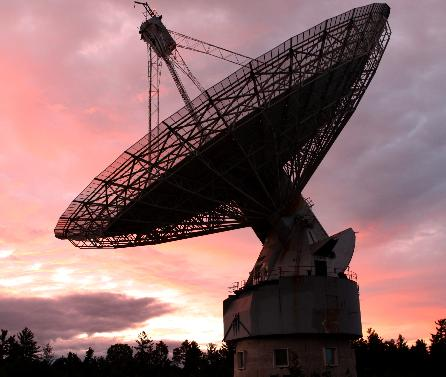
\includegraphics[width=4.4in]{Figures/IMG-7749-ARO-crop.JPG}

\frame{
\vspace{-0.5in}
\begin{center}  
%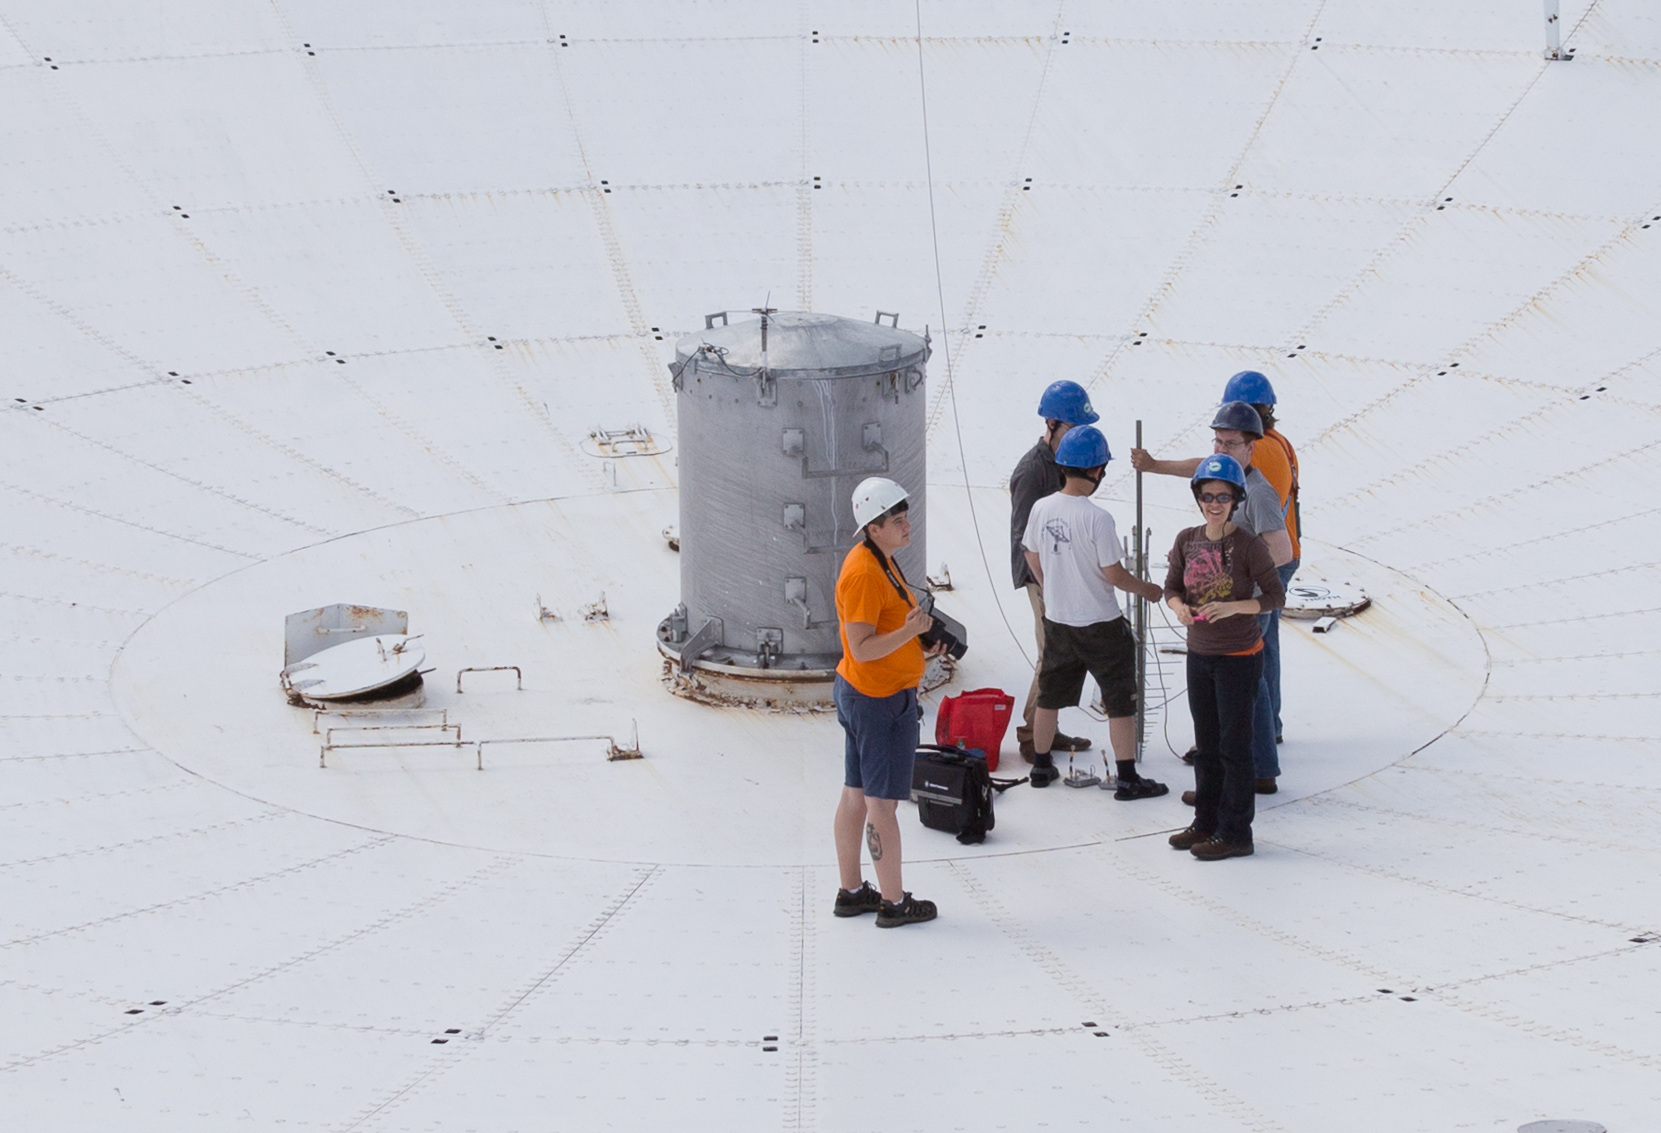
\includegraphics[width=4.4in]{Figures/IMG-0438-by-Andre-cropped.jpg}
\end{center}
\begin{picture}(320,250)
\put(-35,45){
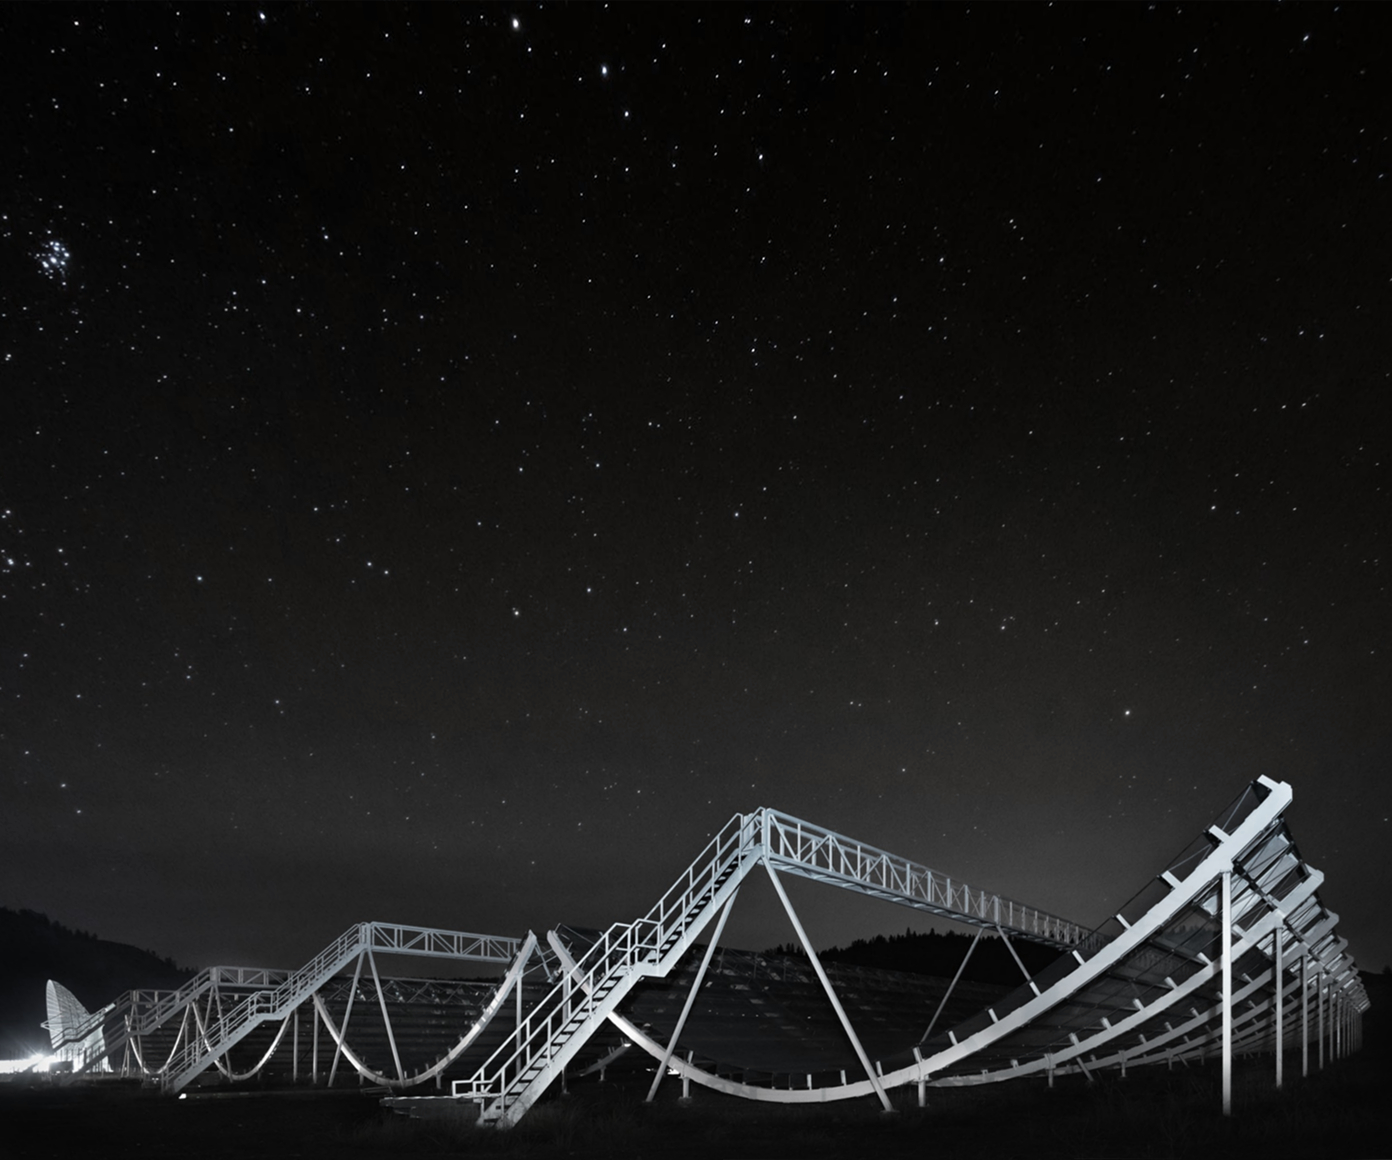
\includegraphics[width=5.1in]{Figures/andre_night_squared_DSC2890.jpg}}
\end{picture}
\vspace{-4in}
\\
image credit: Andre Recnik
\\
\vspace{1in}
\titlepage
}


%\section*{Introduction}
\section{Introduction}

\begin{comment}
  \subsection{Outline}

  \frame{
    \frametitle{Outline}
    \tableofcontents
  }
\end{comment}

  \frame{
    \frametitle{Overview}
    \begin{itemize}
      \item New CHIME results: low frequncy FRB's, repeater
      \item challenges to theory: energetics, coherent emission
      \item what might FRB's be?
      \item what are they good for?
      \item Future prospects
    \end{itemize}
    \vspace{-0.5in}\hspace{2in}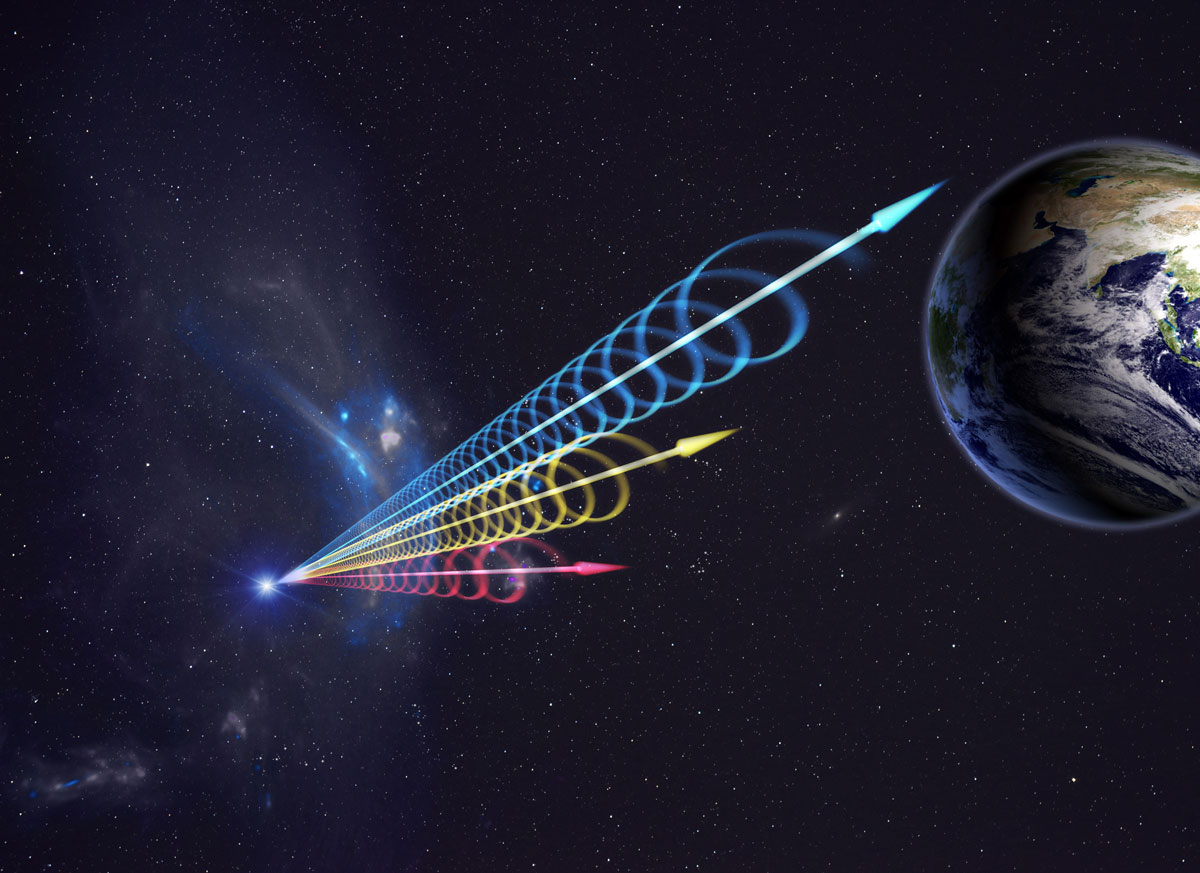
\includegraphics[width=0.6\textwidth]{Figures/imagesnon-gallery2015c-blue12-02-Fast-Radio-BurstsFRB_nrao.jpg}
{\tiny image image credit: Jingchuan Yu, Beijing Planetarium}
  }


  \frame{
    \frametitle{Brief History of FRBs}
    \begin{itemize}
      \item first discovered in 2007, FRB010724
      \item faced with skepticism until 2013 when 4 more were
        confirmed, exhibiting scattering (Thornton et al)
      \item rotation measure and two-screen plasma lensing discovered in 110523 (Masui et al, 2013)
      \item repeater 121102 (Spitler et al 2016)
      \item with high RM ($10^5$)
    \end{itemize}
    \vspace{-0.5in}\hspace{2in}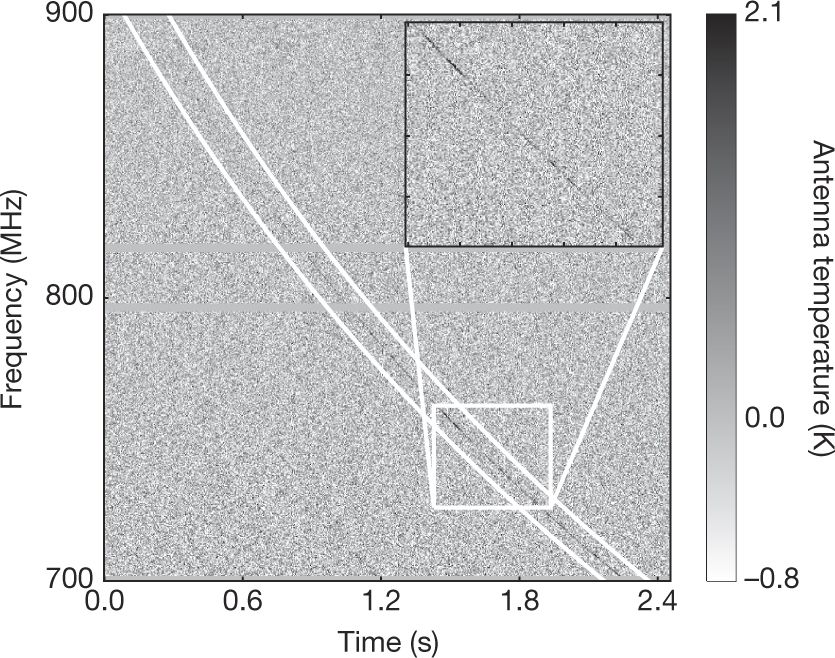
\includegraphics[width=0.6\textwidth]{Figures/nature15769-f1.jpg}
  }


  \frame{
    \frametitle{CHIME-FRB}
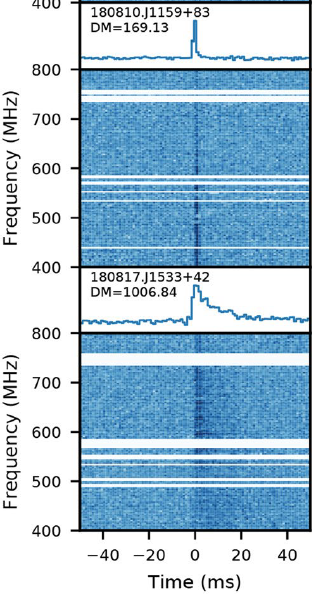
\includegraphics[width=0.35\textwidth]{Figures/chime-frb-precomissioning.png} 
  }

  \frame{
    \frametitle{R2}
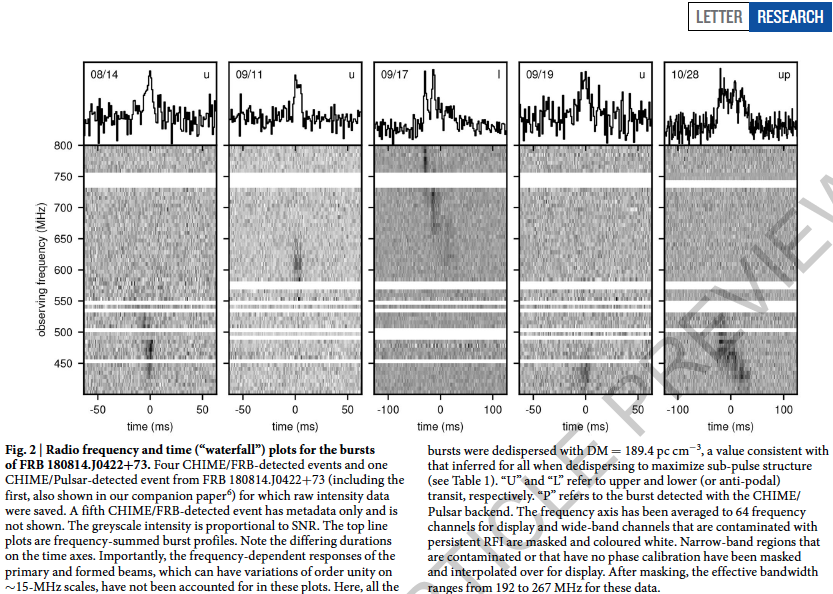
\includegraphics[width=0.9\textwidth]{Figures/chime-R2.png} 
  }

\frame{
    \frametitle{What have we learned?}
    \begin{itemize}
      \item CHIME has unmatched follow-up capability
      \item uncommon repetition is common, perhaps all FRBs repeat
      \item R2 also shows complex narrow frequency-time structure:
        challenge for theory.
      \item many FRB's bright and weakly scattered at bottom of CHIME
        band (400 MHz): excellent probe of plasma propagation effects
      \item 
    \end{itemize}
}




\section{Lensing}

\frame{
    \frametitle{Plasma Lensing}
    \begin{itemize}
      \item galactic scintillation (plasma lensing) provides micro arcsecond probe of
        FRB environment
      \item $\lambda^4$ scattering dependence must be near FRB source:
        not intervener (Vedantham and Phinney)  or IGM
      \item may be source of spectral/temporal structure
    \end{itemize}
}


  \frame{
    \frametitle{Black Widow PSR B1957+20}
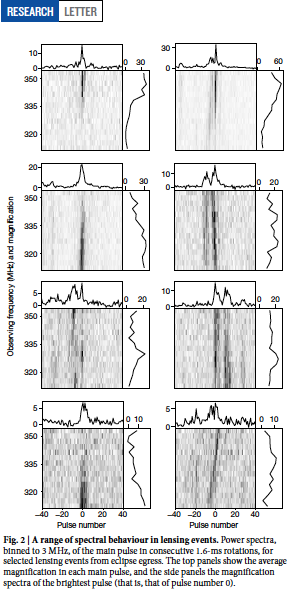
\includegraphics[width=0.35\textwidth]{Figures/black-widow.png}
\vspace{0.5in}
\tiny Main+ 2018
  }


  \frame{
    \frametitle{Grazing incidence}
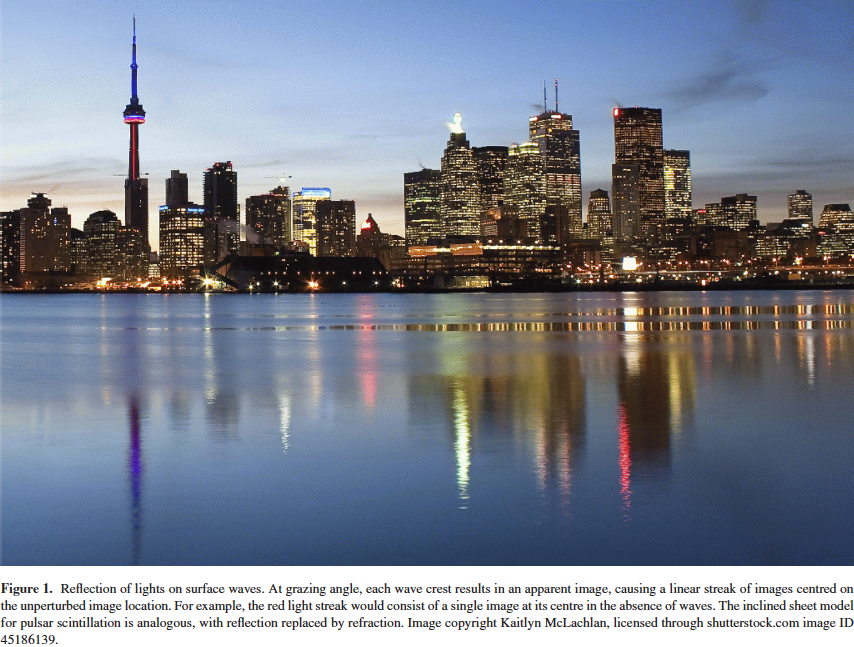
\includegraphics[width=0.9\textwidth]{Figures/toronto.png}
  }


\frame{
    \frametitle{Interference}
    \begin{itemize}
      \item Goldreich Sridhar 2006: refractive images generically
        interfere, e.g. double slit
      \item leads to scintillation scaling $\Delta \nu\propto \nu^{-4}$
      \item projected density caustics: Snell's law diverges
      \item statistics of alignment: rare alignments dominate
        lensing/scattering
      \item use ISM as giant billion km telescope!
    \end{itemize}

\tiny (from wikipedia)

\vspace{-0.5in}\hspace{2.55in}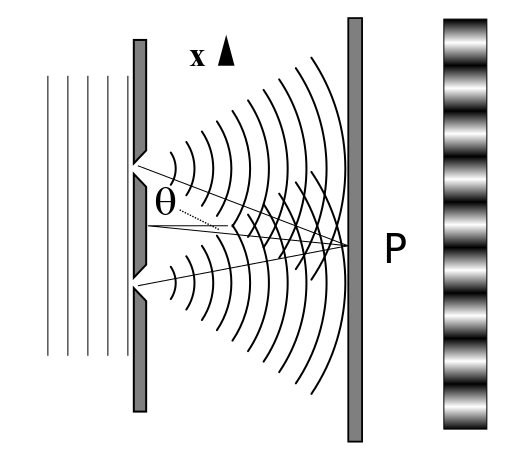
\includegraphics[width=0.4\textwidth]{Figures/Doubleslit.png}
}

\frame{
    \frametitle{Magnetism}
    \begin{itemize}
      \item ISM: (almost) perfect conductor (not superconductor)
      \item local lowest energy state is straight field
      \item impeded by topological entanglement (Braitwaite++ 2004++),
        Gruzinov 2009
      \item originally proposed for Ap stars and white dwarfs
    \end{itemize}
    \vspace{-0.1in}\hspace{3in}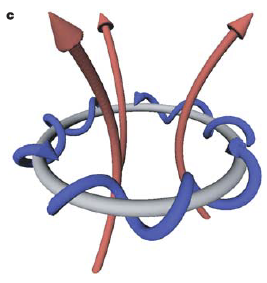
\includegraphics[width=0.3\textwidth]{Figures/braithwaite.png}
}


  \frame{
    \frametitle{Current Sheets}
    \begin{itemize}
      \item magnetic field directional change is exact solution to MHD
        equilibrium: topological domain boundaries
      \item stability unknown, meta-stable (Sweet-Parker 1957+) or unstable (tearing
        mode, Petscheck 1964, +++)
      \item proposed as source of scattering (Goldreich-Sridhar 2006,
        Pen-Levin 2014)
    \end{itemize}
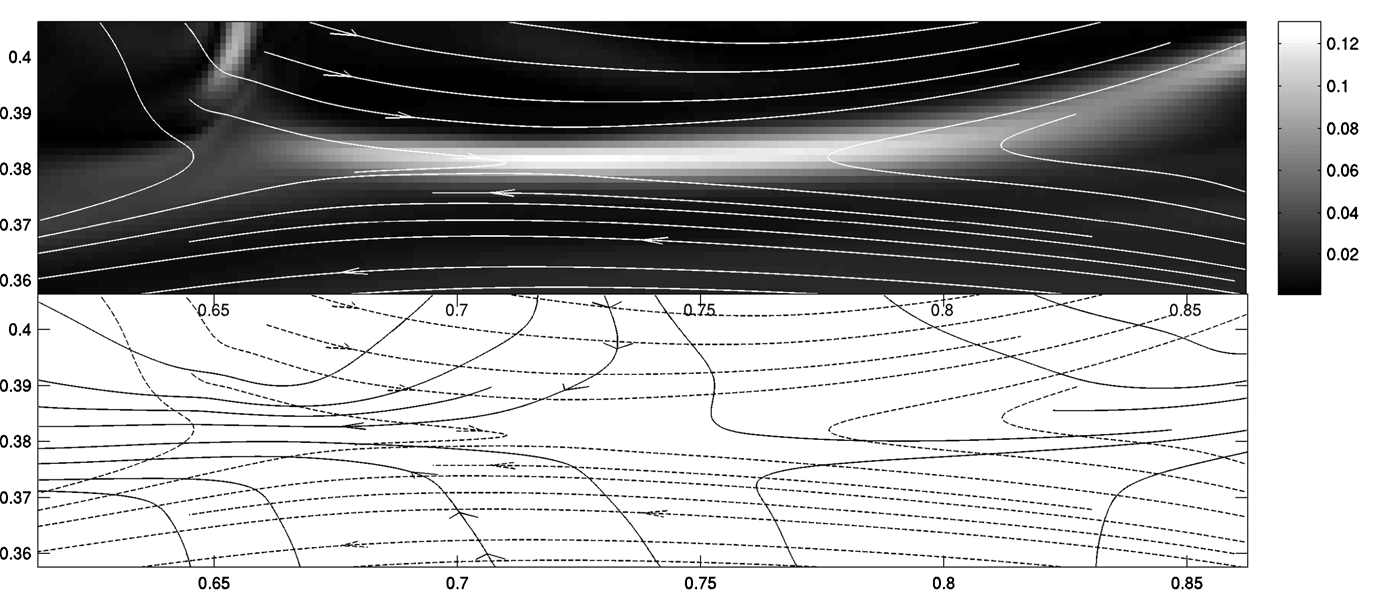
\includegraphics[width=0.9\textwidth]{Figures/reconnection.png} \tiny (Pang+2011)
  }

  \frame{
    \frametitle{Revisit}
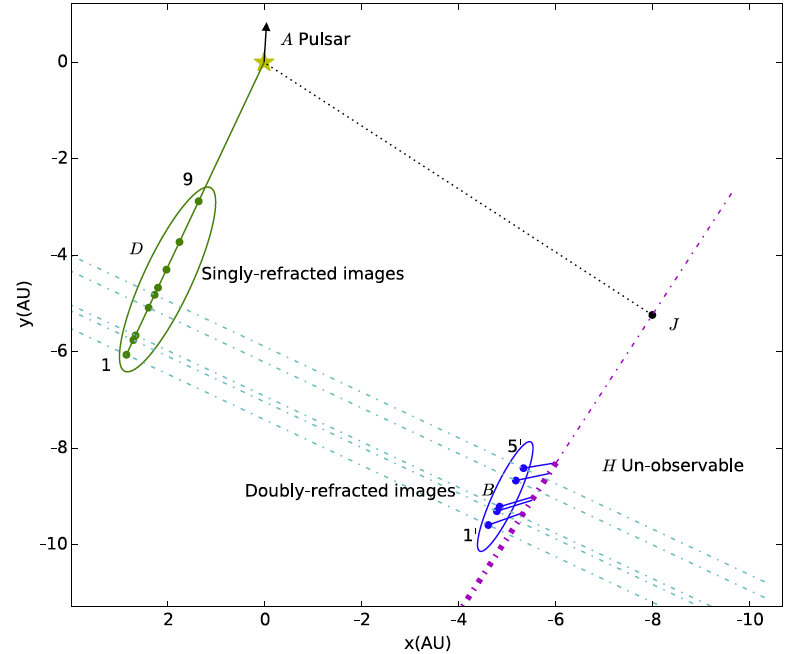
\includegraphics[width=0.8\textwidth]{Figures/liu-lens.png} \tiny
Brisken+2010, Liu+Pen 2016
  }


  \frame{
    \frametitle{Lensing}
    \begin{itemize}
      \item underdense $\longrightarrow$ convergent
      \item overdense $\longrightarrow$ divergent
      \item fold caustic $\longrightarrow$ violate odd image theorem
      \item only one image per wave period, not 4
      \item Simard+UP 2018
    \end{itemize}
\vspace{-0.75in}\hspace{3.5in}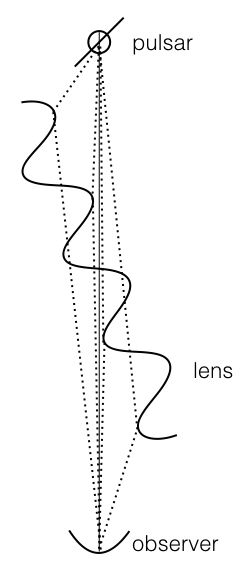
\includegraphics[width=0.25\textwidth]{Figures/convergent_geometry.jpeg}
  }
  \frame{
    \frametitle{Applications}
    \begin{itemize}
      \item cosmic telescope: picoarcsecond astrometry of magnetospheres
      \item measured 1km deflection of PSR B0834+06 emission, initial
        results for crab, black widow
      \item potential for precision distances to pulsars, increased
        PTA sensitivity, accurate GW localization.
    \end{itemize}
  }
 


  \frame{
    \frametitle{Black Widow PSR B1957+20}
    \begin{itemize}
    \item first 'black widow' pulsar: ms pulsar w/ brown dwarf companion
    \item detection of 'cosmic microscope' effects: plasma lensing
      caustics
    \item under {\it Nature} press embargo
    \end{itemize}
%\vspace{-0.3in}%\hspace{1.8in} 
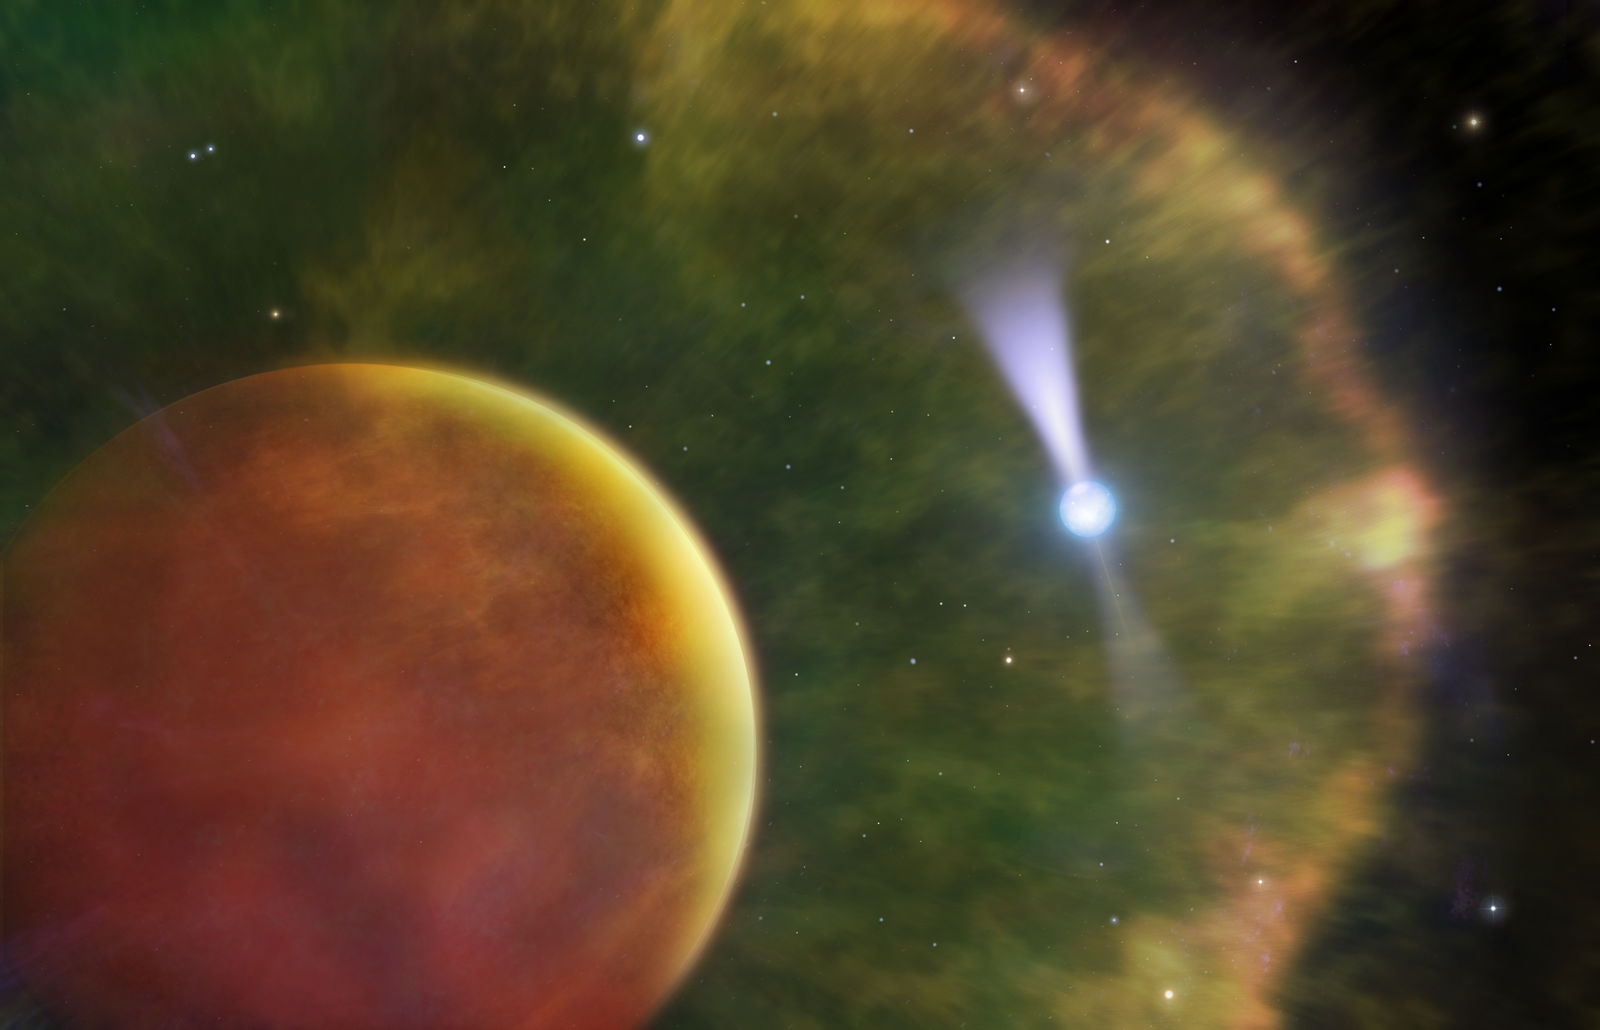
\includegraphics[width=0.6\textwidth]{Figures/1600px-Black_Widow_Binary.jpg}
\vspace{0.5in}
\tiny illustration by Mark Garlick
  }
  \frame{
    \frametitle{Microscope}
    \begin{itemize}
    \item Strong plasma lensing at eclipse egress: up to 100x     
    \item chromatic caustics
    \item resolve interpulse
    \end{itemize}
\vspace{-0.3in}\hspace{1.8in} 
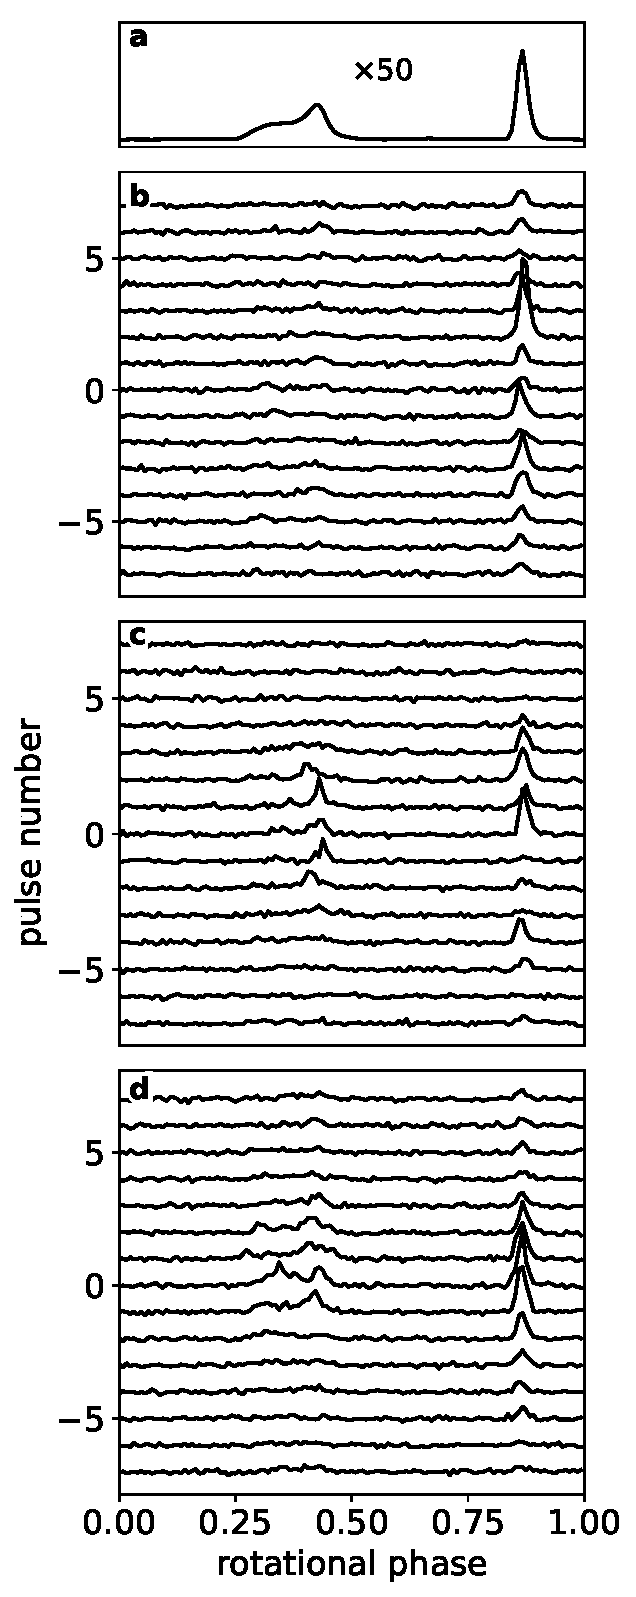
\includegraphics[width=0.25\textwidth]{Figures/ResolvedPulses.pdf}
\vspace{0.5in}
  }

  \frame{
    \frametitle{Applications}
    \begin{itemize}
    \item measure baryon content through cross correlation (McQuinn 2014)
    \item probe extragalactic plasma lensing, magnetic fields
    \item coherent probe of space time, strain $h\sim $ns/Gpc$ \sim 10^{-27}$
    \end{itemize}
  }




  \frame{
    \frametitle{Future}
    \begin{itemize}
      \item Observational:
      \item interferometric array localization: ASKAP, VLA, etc
      \item blind VLBI-localization: CHIME-ARO-GBT
      \item more ambitious localizing surveys: CHIME++, SII
      \item Theory:
      \item coherent emission with narrow frequency structure
      \item Lensing catastrophe theory
    \end{itemize}
  }


  \frame{
    \frametitle{Conclusion}
    \begin{itemize}
      \item CHIME-FRB: new discovery window
      \item FRB challenge: mechanism, uses
        
    \end{itemize}
  }

\end{document}
